\documentclass{beamer}
\usepackage{suesbeamer}
\usepackage{enumerate}
\usepackage{indentfirst}
\usepackage{subfig}
\usepackage{multirow}
\usepackage{booktabs}
\usepackage[numbers,sort&compress]{natbib}
\setcitestyle{square,super}
\setlength{\parindent}{2em}
% 设置插入的表格
\usepackage{tabularx,array}
%% 长表格
\usepackage{longtable}
\usepackage{threeparttable}

%%不需要的内容可以删除掉
\usepackage{tipa}
\usepackage{hologo}
\renewcommand{\TeX}{\hologo{TeX}}
\renewcommand{\LaTeX}{\hologo{LaTeX}}
\newcommand{\BibTeX}{\hologo{BibTeX}}
\newcommand{\XeTeX}{\hologo{XeTeX}}
\newcommand{\pdfTeX}{\hologo{pdfTeX}}
\newcommand{\LuaTeX}{\hologo{LuaTeX}}
\renewcommand{\CTeX}{C\TeX}
\newcommand{\MiKTeX}{\hologo{MiKTeX}}
\newcommand{\MacTeX}{Mac\hologo{TeX}}
\newcommand{\beamer}{\textsc{beamer}}
\newcommand{\XeLaTeX}{\hologo{Xe}\kern-.13em\LaTeX{}}
\newcommand{\pdfLaTeX}{pdf\LaTeX{}}
\newcommand{\LuaLaTeX}{Lua\LaTeX{}}


\author{XXXX}
\title{基于XXXXX技术研究}
\subtitle{开题/中期/结题答辩报告}
\institute{上海工程技术大学电子电气工程学院}
\date{\number\year 年 \number\month 月}

% defs
\def\cmd#1{\texttt{\color{red}\footnotesize $\backslash$#1}}
\def\env#1{\texttt{\color{blue}\footnotesize #1}}
\definecolor{deepblue}{rgb}{0,0,0.5}
\definecolor{deepred}{rgb}{0.6,0,0}
\definecolor{deepgreen}{rgb}{0,0.5,0}
\definecolor{halfgray}{gray}{0.55}

\lstset{
    basicstyle=\ttfamily\small,
    keywordstyle=\bfseries\color{deepblue},
    emphstyle=\ttfamily\color{deepred},    % Custom highlighting style
    stringstyle=\color{deepgreen},
    numbers=left,
    numberstyle=\small\color{halfgray},
    rulesepcolor=\color{red!20!green!20!blue!20},
    frame=shadowbox,
}
\begin{document}
\kaishu
\begin{frame}
    \titlepage
    \begin{figure}[htpb]
        \begin{center}
            
\includegraphics[width=0.2\linewidth]{sues-logo.jpg}
        \end{center}
    \end{figure}
\end{frame}

\begin{frame}
    \frametitle{目录}
    \tableofcontents[sectionstyle=show,subsectionstyle=show/shaded/hide,subsubsectionstyle=show/shaded/hide]
\end{frame}


\section{选题背景}
\begin{frame}{选题来源}
    这里可以将自己的选题来源说明一下,尽量突出主体,行文简洁,标准。
    
    当然在PPT中不能使用太多的字数,主要是为汇报自己当前任务和最后结题的结果等等。
\end{frame}

\section{Latex 排版工具介绍}

\begin{frame}
    \frametitle{\TeX\ 与 \LaTeX\ }
    \begin{columns}[T]
        \column{.8\textwidth}
        \begin{itemize}
            \item \TeX\ (\textipa{/'tEx/},
            \textipa{/'tEk/})
            \begin{itemize}
                \item 最初由 高德纳 (Donald E.~Knuth) 于 1978 年开发的排版系统
                \item 名称源自 technology 的希腊语词根 $\tau\varepsilon\chi$ \par
                    发音接近“泰赫”,而非“泰克斯”
                \item 最新版本为 \TeX\ 3.141592653(2021年1月)\href{https://tex.stackexchange.com/questions/581118/whats-new-in-tex-version-3-141592653}
                \item 漂亮、美观、稳定、通用
                \item 尤其擅长数学公式排版
            \end{itemize}
            \item \LaTeX\ (\textipa{/'la:tEx/}, \textipa{/'leItEk/})
            \begin{itemize}
                \item Leslie Lamport 开发的一种 \TeX{} 格式
                \item 在 \TeX 的基础上提供宏包, 降低使用门槛
                \item 极其丰富的宏包,提供扩展功能
                \item 广泛用于学术界,期刊会议论文模板
                \item 大学学位论文模板,如 
            \end{itemize}
        \end{itemize}
        \column{.2\textwidth}
        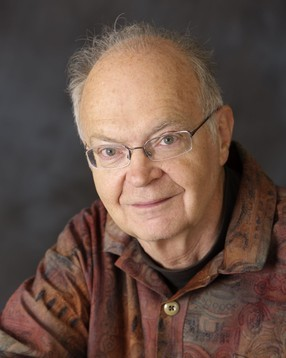
\includegraphics[height=.3\textheight]{Knuth.jpg}

        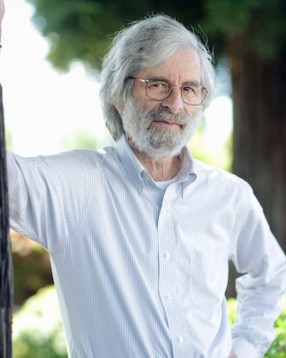
\includegraphics[height=.3\textheight]{Lamport.jpg}
    \end{columns}
\end{frame}

\section{研究内容和创新点}

\begin{frame}{存在的问题}
    对于XXXX的研究过程中,存在以下几方面问题:
    \begin{itemize}
        \item 这里可以将自己当中存在的一些问题列举出来;
        \item 怎么解决的方案可以列举出来;
        \item 这也是一个非常好的方法。
    \end{itemize}
\end{frame}



\begin{frame}{研究内容}
    基于以上的问题,我们提出了以下几种解决方案:
    \begin{itemize}
        \item 方案一;
        \item 方案二;
        \item 方案三
    \end{itemize}
\end{frame}

\begin{frame}{研究意义}
    由于XXX领域存在上述的一些问题,所以这里列举出以下的几个研究的意义
    \begin{itemize}
        \item 增强XXXXX研究的可行性;
        \item 增强XXX模型的适用性;
        \item 为XXXX奠定基础。
    \end{itemize}
\end{frame}

\begin{frame}{创新点}
    本设计主要的创新有以下三点
    \begin{itemize}
        \item \textbf{创新点一}
        \item \textbf{创新点二}
        \item \textbf{创新点三}
        \item \textbf{创新点四}
    \end{itemize}
\end{frame}

\begin{frame}{已有工作基础}
    这里写出自己的已有的工作内容等等。\citet{LiuBo2007}提出了XXX模型,
    \cite{2016Neural,2005Unsupervised}文献中也提及到很多。
    \citet{MengHongyun2008}也提出了一些相应的模型。
\end{frame}

\section{研究方法与解决方案}

\begin{frame}{latex和 Word 对比}
    术业有专攻,评价需客观!
    \begin{table}[h]
      \centering
      %\rowcolors{1}{blue!30}{white!20}
      \begin{tabular}{|c|c|}
        Microsoft\textsuperscript{\textregistered}  Word & \LaTeX \\
        \hline
        字处理工具 & 专业排版软件 \\
        容易上手,简单直观 & 容易上手 \\
        所见即所得 & 所见即所想,所想即所得 \\
        高级功能不易掌握 & 进阶难,但一般用不到 \\
        处理长文档需要丰富经验 & 和短文档处理基本无异 \\
        花费大量时间调格式 & 无需担心格式,专心作者内容 \\
        公式排版差强人意 & 尤其擅长公式排版 \\
        二进制格式,兼容性差 & 文本文件,易读、稳定 \\
        付费商业许可 & 自由免费使用 \\
      \end{tabular}
    \end{table}
\end{frame}



\section{参考文献}
\begin{frame}
    \bibliographystyle{gbt7714-2005-numerical}
    \nocite{*} 
    \bibliography{reference}
\end{frame}

\begin{frame}
    \begin{center}
        {\Huge\calligra Thanks!}
    \end{center}
    \begin{center}
        {\Large\kaishu{谢谢聆听!请各位老师提出意见批评指正}}
    \end{center}
\end{frame}

\end{document}
